\documentclass[hidelinks,12pt]{article}
\usepackage[left=0.25cm,top=1cm,right=0.25cm,bottom=1cm]{geometry}
%\usepackage[landscape]{geometry}
\textwidth = 20cm
\hoffset = -1cm
\usepackage[utf8]{inputenc}
\usepackage[spanish,es-tabla]{babel}
\usepackage[autostyle,spanish=mexican]{csquotes}
\usepackage[tbtags]{amsmath}
\usepackage{nccmath}
\usepackage{amsthm}
\usepackage{amssymb}
\usepackage{mathrsfs}
\usepackage{graphicx}
\usepackage{subfig}
\usepackage{standalone}
\usepackage[outdir=./Imagenes/]{epstopdf}
\usepackage{siunitx}
\usepackage{physics}
\usepackage{color}
\usepackage{float}
\usepackage{hyperref}
\usepackage{multicol}
%\usepackage{milista}
\usepackage{anyfontsize}
\usepackage{anysize}
%\usepackage{enumerate}
\usepackage[shortlabels]{enumitem}
\usepackage{capt-of}
\usepackage{bm}
\usepackage{relsize}
\usepackage{placeins}
\usepackage{empheq}
\usepackage{cancel}
\usepackage{wrapfig}
\usepackage[flushleft]{threeparttable}
\usepackage{makecell}
\usepackage{fancyhdr}
\usepackage{tikz}
\usepackage{bigints}
\usepackage{scalerel}
\usepackage{pgfplots}
\usepackage{pdflscape}
\pgfplotsset{compat=1.16}
\spanishdecimal{.}
\renewcommand{\baselinestretch}{1.5} 
\renewcommand\labelenumii{\theenumi.{\arabic{enumii}})}
\newcommand{\ptilde}[1]{\ensuremath{{#1}^{\prime}}}
\newcommand{\stilde}[1]{\ensuremath{{#1}^{\prime \prime}}}
\newcommand{\ttilde}[1]{\ensuremath{{#1}^{\prime \prime \prime}}}
\newcommand{\ntilde}[2]{\ensuremath{{#1}^{(#2)}}}

\newtheorem{defi}{{\it Definición}}[section]
\newtheorem{teo}{{\it Teorema}}[section]
\newtheorem{ejemplo}{{\it Ejemplo}}[section]
\newtheorem{propiedad}{{\it Propiedad}}[section]
\newtheorem{lema}{{\it Lema}}[section]
\newtheorem{cor}{Corolario}
\newtheorem{ejer}{Ejercicio}[section]

\newlist{milista}{enumerate}{2}
\setlist[milista,1]{label=\arabic*)}
\setlist[milista,2]{label=\arabic{milistai}.\arabic*)}
\newlength{\depthofsumsign}
\setlength{\depthofsumsign}{\depthof{$\sum$}}
\newcommand{\nsum}[1][1.4]{% only for \displaystyle
    \mathop{%
        \raisebox
            {-#1\depthofsumsign+1\depthofsumsign}
            {\scalebox
                {#1}
                {$\displaystyle\sum$}%
            }
    }
}
\def\scaleint#1{\vcenter{\hbox{\scaleto[3ex]{\displaystyle\int}{#1}}}}
\def\bs{\mkern-12mu}


\title{Problemas de tipo Sturm-Liouville \\ \large {Tema 3 - Bases completas y ortogonales}\vspace{-3ex}}

\author{M. en C. Gustavo Contreras Mayén}
\date{ }

\pagestyle{fancy}
\fancyhf{}
\rhead{Curso MAF}
\lhead{\leftmark}
\rfoot{\thepage}
\setlength{\headheight}{16pt}%


\begin{document}
\maketitle
\fontsize{14}{14}\selectfont
\tableofcontents
\newpage

%Ref. Herman (2015)  - Sturm-Liouville 
\section{Problemas de tipo Sturm-Liouville.}

Hemos visto que las funciones trigonométricas y que algunas las funciones especiales son las soluciones de ecuaciones diferenciales. Estas soluciones dan conjuntos ortogonales de funciones que se pueden utilizar para representar funciones en expansiones de series de Fourier generalizadas.
\par
Al mismo tiempo, sería interesante generalizar las técnicas que usamos por primera vez para resolver la ecuación de calor con el fin de resolver problemas más generales de valores iniciales (VI) o con condiciones de frontera (CDF). Es decir, usamos la separación de variables para separar la ecuación diferencial parcial dada en un conjunto de ecuaciones diferenciales ordinarias. Un subconjunto de esas ecuaciones nos proporciona un conjunto de problemas de valores en la frontera cuyas funciones propias son útiles para representar soluciones de la ecuación diferencial parcial. Con suerte, esas soluciones constituirán una base útil en algún espacio funcional.
\par
Una clase de problemas a la que pertenecen estos ejemplos anteriores, son \emph{los problemas de valores propios de Sturm-Liouville}. Estos problemas involucran \emph{operadores autoadjuntos} (diferenciales) que juegan un papel importante en la teoría espectral de operadores lineales y la existencia de las funciones propias necesarias para resolver los interesantes problemas de física descritos por los problemas de VI o CDF anteriores.

\subsection{Operadores de Sturm-Liouville.}

En física, muchos problemas surgen en forma de problemas de CDF que involucran ecuaciones diferenciales ordinarias de segundo orden. Por ejemplo, exploraremos la ecuación de onda y la ecuación de calor en tres dimensiones. Separar la dependencia del tiempo conduce a un problema de valor límite tridimensional en ambos casos. Una mayor separación de variables conduce a un conjunto de problemas de valores de frontera que involucran ecuaciones diferenciales ordinarias de segundo orden.
\par
En general, podríamos obtener ecuaciones de la forma:
\begin{align}
a_{2} (x) \, \sderivada{y} + a_{1} (x) \, \pderivada{y} + a_{0} (x) \, y = f(x)
\label{eq:ecuacion_04_01}
\end{align}
sujeta a CDF. Podemos escribir una ecuación de este tipo en forma de un operador definiendo el \emph{operador diferencial}:
\begin{align*}
L - a_{2} (x) \, D^{2} + a_{1} (x) \, D + a_{0} (x)
\end{align*}
donde $D = \dv*{x}$. Entonces, la ecuación (\ref{eq:ecuacion_04_01}) toma la forma:
\begin{align*}
L \, y = f
\end{align*}
Veremos que estas ecuaciones se pueden resolver usando \emph{expansiones de funciones propias}. Es decir, buscamos soluciones al problema de los valores propios:
\begin{align*}
L \, \phi = \lambda \, \phi
\end{align*}
con CDF homogéneas en $\phi$ y luego buscar una solución del problema no homogéneo: $L \, y = f$, como una expansión sobre estas funciones propias. Formalmente, hacemos que:
\begin{align*}
y (x) = \nsum_{n=1}^{\infty} c_{n} \, \phi_{n} (x)
\end{align*}
Sin embargo, no se garantiza un buen conjunto de funciones propias. Necesitamos un conjunto apropiado para formar una base en el espacio funcional. Además, sería bueno tener ortogonalidad para que podamos resolver fácilmente los coeficientes de expansión.
\par
Resulta que cualquier operador diferencial lineal de segundo orden puede convertirse en un operador que posea las propiedades adecuadas (autoadjuntas) para llevar a cabo este procedimiento. El operador resultante se denomina \emph{operador Sturm-Liouville}. Revisaremos algunas de las propiedades de estos operadores y ver cómo se aplican.
\par
Se define el operador Sturm-Liouville como:
\begin{align}
\mathcal{L} = \dv{x} \, p(x) \, \dv{x} + q(x)
\label{eq:ecuacion_04_02}
\end{align}

El problema de valores propios de tipo Sturm-Liouville está dado por la siguiente ecuación diferencial:
\begin{align*}
\mathcal{L} \, y = - \lambda \, \sigma(x) \, y
\end{align*}
o de manera equivalente:
\begin{align}
\dv{x} \left( p(x) \, \dv{x} \right) + q(x) \, y + \lambda \, \sigma (x) \, y = 0
\label{eq:ecuacion_04_03}
\end{align}
para $x \, \in \, (a, b)$, $y = y (x)$, más las CDF. Se supone que las funciones $p (x)$, $\pderivada{p} (x)$, $q (x)$ y $\sigma (x)$ son continuas en $(a, b)$ y $p (x) > 0$, $\sigma (x) > 0$ en $[a , b]$. Si el intervalo es finito y estas suposiciones sobre los coeficientes son verdaderas en $[a, b]$, entonces se dice que el problema es un \emph{problema regular de Sturm-Liouville}. De lo contrario, se denomina \emph{problema singular de Sturm-Liouville}.
\par
También necesitamos imponer un conjunto de CDF homogéneas:
\begin{align}
\begin{aligned}
\alpha_{1} \, y(a) + \beta_{1} \, \pderivada{y} (a) &= 0 \\[0.5em]
\alpha_{2} \, y(b) + \beta_{2} \, \pderivada{y} (b) &= 0
\end{aligned}
\label{eq:ecuacion_04_04}
\end{align}
Las $\alpha$ y $\beta$ son constantes. Para diferentes valores, se tienen tipos especiales de condiciones de contorno. Para $\beta_{i} = 0$, tenemos las llamadas condiciones de frontera de Dirichlet, es decir, $y (a) = 0$ y $y (b) = 0$. Para $\alpha_{i} = 0$, se tienen las condiciones de frontera de Neumann. En este caso, $\pderivada{y} (a) = 0$ y $\pderivada{y} (b) = 0$.
\par
En términos del ejemplo de la ecuación de calor, las condiciones de Dirichlet corresponden a mantener una temperatura fija en los extremos de la varilla. Las condiciones de frontera de Neumann corresponderían a ningún flujo de calor a través de los extremos, o condiciones de aislamiento, ya que no habría gradiente de temperatura en esos puntos. Las condiciones de contorno más generales permiten límites parcialmente aislados.
\par
Otro tipo de CDF que se encuentra a menudo es la \emph{condición de frontera periódica}. Considera una varilla calentada que se ha doblado para formar un círculo. Entonces, los dos puntos finales son físicamente iguales. \iffalse \footnote{Este problema se encuentra en el Examen del Tema 2.} \fi Entonces, esperaríamos que la temperatura y el gradiente de temperatura coincidieran en esos puntos. Para este caso escribimos $y (a) = y (b)$ y $\pderivada{y} (a) = \pderivada{y} (b)$. Los problemas de valores límite que utilizan estas condiciones deben manejarse de manera diferente a las condiciones homogéneas anteriores. Estas condiciones conducen a diferentes tipos de funciones propias y valores propios.
\par
Como se mencionó anteriormente, las ecuaciones de la forma (\ref{eq:ecuacion_04_01}) se presentan con frecuencia. Ahora mostramos que cualquier operador lineal de segundo orden se puede poner en la forma del operador de Sturm-Liouville. En particular, la ecuación (\ref{eq:ecuacion_04_01}) se puede escribir de la forma:
\begin{align}
\dv{x} \left( p(x) \, \dv{x} \right) + q(x) \, y =  F(x)
\label{eq:ecuacion_04_05}
\end{align}

Otra forma de expresar esto se proporciona en el teorema: La prueba de esto es sencilla, como se verá pronto. Consideremos primero la ecuación (\ref{eq:ecuacion_04_01}) para el caso de que $a_{1} (x) = \pderivada{a}_{2} (x)$. Entonces, podemos escribir la ecuación en una forma en la que los dos primeros términos se combinen:
\begin{align}
\begin{aligned}
f(x) &= a_{2} (x) \, \sderivada{y} + a_{1} (x) \, \pderivada{y} + a_{0} (x) \, y = \\[0.5em]
&= \big[ a_{2} (x) \, \pderivada{y} \, \big]^{\prime} + a_{0} (x) \, y
\end{aligned}
\label{eq:ecuacion_04_06}
\end{align}
La ecuación resultante está ahora en la forma de Sturm-Liouville. Simplemente identificamos $p(x) = a_{2} (x)$ y $q (x) = a_{0} (x)$.
\par
No todas las ecuaciones diferenciales de segundo orden son tan sencillas de convertir. Considera la ecuación diferencial:
\begin{align*}
x^{2} \, \sderivada{y} + x \, \pderivada{y} + 2 \, y = 0
\end{align*}
En este caso $a_{2} (x) = x^{2}$ y $\pderivada{a}_{2} (x) = 2 \, x \neq a_{1} (x)$. Entonces, esto no viene al caso. Sin embargo, podemos cambiar el operador en esta ecuación, $x^{2} \, D + x \, D$, a un operador de Sturm-Liouville, $D \, p (x) \, D$ para un $p (x)$ que depende de los coeficientes $x^{2}$ y $x$.
\par
En el operador de Sturm Liouville, los términos de la derivada se agrupan en una derivada \enquote{perfecta}, $D \, p (x) \, D$. Esto es similar cuando se resuelven ecuaciones lineales de primer orden, se busca un factor integrador. Es posible hacer lo mismo aquí: buscamos una función $\mu (x)$ que podamos multiplicar con la ec. (\ref{eq:ecuacion_04_01}) para que pueda escribirse en la forma de Sturm-Liouville.
\par
Primero dividimos entre $a_{2} (x)$, obteniendo:
\begin{align*}
\sderivada{y} + \dfrac{a_{1}(x)}{a_{2}(x)} \, \pderivada{y} + \dfrac{a_{0}(x)}{a_{2}(x)} \, y = \dfrac{f(x)}{a_{2}(x)}
\end{align*}

El siguiente paso es multiplicar la ecuación diferencial por $\mu$:
\begin{align*}
\mu(x) \, \sderivada{y} + \mu(x) \, \dfrac{a_{1}(x)}{a_{2}(x)} \, \pderivada{y} + \mu(x) \, \dfrac{a_{0}(x)}{a_{2}(x)} \, y = \mu(x) \, \dfrac{f(x)}{a_{2}(x)}
\end{align*}

Los dos primeros términos ahora se pueden combinar en una derivada exacta $( \mu \, \pderivada{y})^{\prime}$  si el segundo coeficiente es $\pderivada{\mu} (x)$. Por lo tanto, $\mu (x)$ satisface una ecuación diferencial separable de primer orden:
\begin{align*}
\dv{\mu}{x} = \mu (x) \, \dfrac{a_{1}(x)}{a_{2} (x)}
\end{align*}
Esto se resuelve formalmente para dar el factor de integración buscado:
\begin{align*}
\mu (x) = \exp \left( \scaleint{6ex} \, \dfrac{a_{1}(x)}{a_{2}(x)} \dd{x} \right)
\end{align*}
Por tanto, la ecuación original se puede multiplicar por factor:
\begin{align*}
\dfrac{\mu(x)}{a_{2}(x)} = \dfrac{1}{a_{2}(x)} \, \exp \left( \scaleint{6ex} \, \dfrac{a_{1}(x)}{a_{2}(x)} \dd{x} \right)
\end{align*}
para obtener una expresión en forma de Sturm-Liouville.
\par
\noindent
En resumen: La ec. (\ref{eq:ecuacion_04_01}):
\begin{align}
a_{2} (x) \, \sderivada{y} + a_{1} (x) \, \pderivada{y} + a_{0} \, y = f(x)
\label{eq:ecuacion_04_07}
\end{align}
se puede escribir de la forma Sturm-Liouville:
\begin{align}
\dv{x} \left( p(x) \, \dv{x} \right) + q(x) \, y =  F(x)
\label{eq:ecuacion_04_08}
\end{align}
donde:
\begin{align}
\begin{aligned}
p(x) &= \exp \left( \scaleint{6ex} \, \dfrac{a_{1}(x)}{a_{2}(x)} \dd{x} \right) \\[0.5em]
q(x) &= p(x) \, \dfrac{a_{0}(x)}{a_{2}(x)} \\[0.5em]
F(x) &= p(x) \, \dfrac{f(x)}{a_{2}(x)}
\end{aligned}
\label{eq:ecuacion_04_09}
\end{align}

\begin{ejemplo}\label{Ejemplo_01}
Escribe la siguiente EDO2H en la forma de Sturm-Liouville:
\begin{align*}
x^{2} \, \sderivada{y} + x \, \pderivada{y} + 2 \, y = 0
\end{align*}
Podemos multiplicar esta ecuación por:
\begin{align*}
\dfrac{\mu (x)}{a_{2}(x)} = \dfrac{1}{x^{2}} \, \exp \left( \scaleint{6ex} \, \dfrac{\dd{x}}{x} \right) = \dfrac{1}{\pderivada{x}}
\end{align*}
para escribirla en la forma de Sturm-Liouville:
\begin{align*}
x \, \sderivada{y} + \pderivada{y} + \dfrac{2}{x} \, y &= 0 \\[0.5em]
\big( x \, \pderivada{y} \big)^{\prime} +  \dfrac{2}{x} \, y &= 0
\end{align*}
\end{ejemplo}

\section{Propiedades de valores propios de S-L.}

Hay varias propiedades que se pueden probar para el problema de valores propios de Sturm-Liouville (regular) dado por la ec. (\ref{eq:ecuacion_04_03}). Sin embargo, no se probarán todos aquí. Simplemente vamos a enumerar algunos de los hechos importantes y nos centraremos en algunas de las propiedades.
\begin{enumerate}
\item Los autovalores\footnote{La palabra alemana \emph{eigen}, se traduce en español como propio, se uso por primera vez en este contexto por David Hilbert en 1904. Eigen también se ha traducido como inherente, característico o por el prefijo auto-. En español se utiliza el prefijo auto- o propio, siendo característico también en portugués e italiano, pero en otros idiomas en matemática se utiliza la palabra alemana eigen sin conflictos a la referencia.} son reales, contables, ordenados y hay un valor propio más pequeño. Por tanto, podemos escribirlos como $\lambda_{1} < \lambda_{2} < \ldots $ Sin embargo, no hay un valor propio más grande: si $n \to \infty$, $\lambda_{n} \to \infty$.
\item Para cada valor propio $\lambda_{n}$ existe una función propia $\phi_{n}$ con $n - 1$ ceros en $(a, b)$.
\item Las funciones propias que corresponden a diferentes valores de las mismas son ortogonales con respecto a la función de peso, $\sigma (x)$. Al definir el producto interno de $f (x)$ y $g (x)$ como:
\begin{align}
\langle f , g \rangle = \scaleint{6ex}_{\bs a}^{b} f(x) \, g(x) \, \sigma(x) \dd{x}
\label{eq:ecuacion_04_11}
\end{align}
entonces la ortogonalidad de las funciones propias se puede escribir de la forma:
\begin{align}
\langle \phi_{n}, \phi_{m} \rangle = \langle \phi_{n}, \phi_{m} \rangle \, \delta_{nm} \hspace{1.5cm} n, m = 1, 2, \ldots
\label{eq:ecuacion_04_12}
\end{align}

\item El conjunto de funciones propias es completo, es decir, cualquier función suave se puede representar mediante una expansión generalizada de las funciones propias de la serie de Fourier:
\begin{align*}
f(x) \sim \nsum_{n=1}^{\infty} c_{n} \, \phi_{n} (x)
\end{align*}
donde
\begin{align*}
c_{n} = \dfrac{\langle f, \phi_{n} \rangle}{\langle \phi_{n}, \phi_{n} \rangle}
\end{align*}
En realidad, se necesita que $f (x) \in \, L_{\sigma}^{2} (a, b$), el conjunto de funciones de cuadrado integrables sobre $[a, b]$ con la función de peso $\sigma (x)$. Por cuadrado integrable, queremos decir que $\langle f,  f \rangle < \infty$. Se puede demostrar que tal espacio es isomorfo en un espacio de Hilbert, un espacio de producto interno completo. Los espacios de Hilbert juegan un papel especial en la mecánica cuántica\footnote{En el material adicional encontrarás una referencia sobre los espacios de Hilbert y la notación de Dirac, que es de gran importancia en la mecánica cuántica.}.
\item Los valores propios satisfacen el cociente de Rayleigh:
\begin{align*}
\lambda_{n} = \dfrac{- p \, \phi_{n} \, \displaystyle \dv{\phi_{n}}{x} \eval_{b}^{a} + \scaleint{6ex}_{\bs a}^{b} \bigg[ p \left( \dv{\phi_{n}}{x} \right)^{2} - q \, \phi_{n}^{2} \bigg] \dd{x}}{\langle  \phi_{n}, \phi_{n} \rangle} 
\end{align*}
Esto se puede verificar al multiplicar el problema de valores propios:
\begin{align*}
\mathcal{L} \, \phi_{n} = - \lambda_{n} \, \sigma(x) \, \phi_{n}
\end{align*}
por $\phi_{n}$ y luego integrar. Al resolver este resultado para $\lambda_{n}$, se obtiene el cociente de Rayleigh. El cociente de Rayleigh es útil para obtener estimaciones de valores propios y probar algunas de las otras propiedades.
\end{enumerate}

\begin{ejemplo}
Verifica algunas de las propiedades para el siguiente problema de valores propios:
\begin{align*}
\sderivada{y} = - \lambda \, y \hspace{1cm} y(0) = y(\pi) = 0
\end{align*}

Este es un problema que ya se ha visto muchas veces. Las funciones propias para este problema de autovalores\footnote{Como se revisará, podemos hacer referencia de manera indistinta al concepto de funciones y valores propios, así como de autofunciones, autovalores, además de eigenfunciones y eigenvalores, ya que como se comentó en el material adicional de la función delta de Dirac, no hay confusión gramatical al ocupar la palabra \emph{eigen} en español.} son $\phi_{n} (x) = \sin n\, x$, con autovalores $\lambda_{n} = n^{2}$ para $n = 1, 2, \ldots$. Éstas satisfacen las propiedades enumeradas anteriormente.
\par
En primer lugar, los valores propios son reales, contables y ordenados, $1 < 4 < 9 < \ldots$. No hay un valor propio más grande pero hay un primer valor.
\par
Las funciones propias correspondientes a cada valor propio tienen $n -1$ ceros en el intervalo $(0, \pi)$. Esto se comprueba para varias funciones propias en la figura (\ref{fig:figura_04_01}).
\begin{figure}[H]
    \centering
    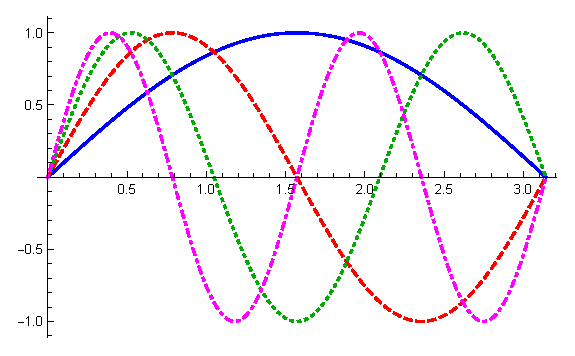
\includegraphics[scale=1.3]{Imagenes/Eigenfunciones_Sin_nx.eps}
    \caption{Gráfica de las funciones propias $\phi_{n} (x) = \sin n \,x$ para $n = 1, 2, 3, 4$.}
    \label{fig:figura_04_01}
\end{figure}
También sabemos que el conjunto $\left\{ \sin n \, x \right\}$ con $n = 1, \ldots, \infty$ es un conjunto ortogonal de funciones básicas de longitud:
\begin{align*}
\norm{\phi_{n}} = \sqrt{\dfrac{\pi}{2}}
\end{align*}
Por lo tanto, el cociente de Rayleigh se puede calcular usando $p(x) = 1$, $q (x) = 0$ y las funciones propias. Está dado entonces por:
\begin{align}
\begin{aligned}[b]
R &= \dfrac{- \phi_{n} \, \pderivada{\phi}_{n} \eval_{0}^{\pi} + \scaleint{6ex}_{\bs 0}^{\pi} \, (\pderivada{\phi}_{n})^{2} \dd{x}}{\dfrac{\pi}{2}} = \\[0.5em]
&= \dfrac{2}{\pi} \scaleint{6ex}_{\bs 0}^{\pi} \left( - n^{2} \, \cos n \, x \right)^{2} \dd{x} = \\[0.5em]
&= n^{2}
\end{aligned}
\label{eq:ecuacion_04_13}
\end{align}
Por lo tanto, conociendo la función propia, el cociente de Rayleigh devuelve los valores propios como se esperaba.
\end{ejemplo}

\begin{ejemplo}
Buscamos las funciones propias del operador que se encuentran en el \textbf{Ejemplo 1}. Es decir, queremos resolver el problema de los valores propios:
\begin{align}
\mathcal{L} \, y = \left( x \, \pderivada{y} \right)^{\prime} + \dfrac{2}{x} \, y = - \lambda \, \sigma \, y
\label{eq:ecuacion_04_14}
\end{align}
sujeta a las CDF:
\begin{align*}
\pderivada{y} (1) = 0, \hspace{1cm} \pderivada{y}(2) = 0
\end{align*}
Tomemos en cuenta que todavía no conocemos quién es la función $\sigma (x)$, pero elegiremos una función adecuada para obtener las soluciones.
\par
\noindent
Expandiendo la derivada, tendremos que:
\begin{align*}
x \, \sderivada{y} + \pderivada{y} + \dfrac{2}{x} \, y = - \lambda \, \sigma \, y
\end{align*}
multiplicamos por $x$ para obtener:
\begin{align*}
x^{2} \, \sderivada{y} + x \, \pderivada{y} + (2 + \lambda \, x \,  \sigma) \, y = 0
\end{align*}
Veamos que si elegimos $\sigma(x) = x^{-1}$, entonces la ecuación se puede expresar como una ecuación de tipo Cauchy-Euler. Entonces tendremos:
\begin{align*}
x^{2} \, \sderivada{y} + x \, \pderivada{y} + (\lambda + 2) \, y = 0
\end{align*}
La ecuación característica es:
\begin{align*}
r^{2} + \lambda + 2 = 0
\end{align*}
Para tener soluciones oscilatorias, se necesita que $\lambda + 2 > 0$. Por lo tanto, la solución general es:
\begin{align}
y(x) = c_{1} \, \cos \left( \sqrt{\lambda + 2} \, \ln \abs{x} \right) + c_{2} \, \sin \left( \sqrt{\lambda + 2} \, \ln \abs{x} \right)
\label{eq:ecuacion_04_15}
\end{align}
Aplicamos las CDF $\pderivada{y}(1) = 0$, obliga que $c_{2} = 0$, esto nos deja:
\begin{align*}
y(x) = c_{1} \, \cos \left( \sqrt{\lambda + 2} \, \ln \abs{x} \right)
\end{align*}
La segunda condición $\pderivada{y}(2) = 0$, nos lleva a:
\begin{align*}
\sin \left( \sqrt{\lambda + 2} \, \ln 2 \right) = 0
\end{align*}
las soluciones no triviales se presentan cuando:
\begin{align*}
\sqrt{\lambda + 2} \, \ln 2 = n \, \pi \hspace{1.5cm} n = 0, 1, 2, \ldots
\end{align*}

Entonces se tiene que las funciones propias para este problema de valores propios son:
\begin{align*}
y_{n}(x) = \cos \left( \dfrac{n \, \pi}{\ln 2} \, \ln x \right), \hspace{1.5cm} 1 \leq x \leq 2
\end{align*}
y los valores propios son:
\begin{align*}
\lambda_{n} = \left( \dfrac{n \, \pi}{\ln 2} \right)^{2} - 2, \hspace{1.5cm} n = 0, 1, 2, \ldots
\end{align*}

\emph{Nota:} Incluimos el caso $n = 0$ porque $y (x) =$ constante, es una solución del caso $\lambda = - 2$. Más específicamente, en este caso la ecuación característica se reduce a $r^{2} = 0$. Por lo tanto, la solución general de esta ecuación de Cauchy-Euler es:
\begin{align*}
y (x) = c_{1} + c_{2} \, \ln \abs{x}
\end{align*}

Haciendo que $\pderivada{y} (1) = 0$, obliga que $c_{2} = 0$. Por lo que $\pderivada{y} (2)$ se anula automáticamente, dejando la solución en este caso como $y(x) = c_{1}$.
\par
Observamos que algunas de las propiedades enumeradas al principio de la sección son válidas para este ejemplo. Los valores propios se consideran reales, contables y ordenados. Hay al menos uno, $\lambda_{0} = -2$. A continuación, se pueden encontrar los ceros de cada función propia en el intervalo $[1, 2]$. Entonces, el argumento del coseno, $\left( \dfrac{n \, \pi}{\ln 2} \, \ln x \right)$, toma valores de $0$ a $n \pi$ para $x \in [1, 2]$. La función coseno tiene $n - 1$ raíces en este intervalo.
\par
La ortogonalidad se revisa como sigue: En la integral usamos el cambio de variable $y = \dfrac{\pi \, \ln x}{\ln 2}$. Esto nos devuelve:
\begin{align}
\begin{aligned}[b]
\langle y_{n}, y_{n} \rangle &= \scaleint{6ex}_{\bs 1}^{2} \, \cos \left( \dfrac{n \, \pi}{\ln 2} \, \ln x \right) \, \cos \left( \dfrac{m \, \pi}{\ln 2} \, \ln x \right) \dfrac{\dd{x}}{x} = \\[0.5em]
&= \dfrac{\ln 2}{\pi} \scaleint{6ex}_{\bs 0}^{\pi} \cos (n \, y) \, \cos (m \, y) \dd{y} = \\[0.5em]
&= \dfrac{\ln 2}{2} \, \delta_{nm}
\end{aligned}
\label{eq:ecuacion_04_16}
\end{align}
\end{ejemplo}
% \section{Ejercicios a cuenta.}

% %Ref. Boyce. 11.1 Problemas 8, 10, 11

% \textbf{Ejercicio a cuenta (27). }  Transforma las siguientes EDO2H a la forma de tipo Sturm-Liouville.
% \begin{enumerate}[label=\roman*)]
% \item Ecuación de Hermite. \hspace{1cm} $\sderivada{y} - 2 \, x \, \pderivada{y} + \lambda \, y = 0$
% \item Ecuación de Laguerrre. \hspace{0.75cm} $x\, \sderivada{y} + (1 - x) \, \pderivada{y} + \lambda \, y = 0$
% \item Ecuación de Chebyshev. \hspace{0.5cm} $(1 - x^{2}) \, \sderivada{y} - x \, \pderivada{y} + \alpha^{2} \, y = 0$
% \end{enumerate}

% %Ref. Boyce 11.2  Problema 3
% \textbf{Ejercicio a cuenta (28). } Determina los valores propios y las funciones propias con las CDF.
% \begin{align*}
% \sderivada{y} + \lambda \, y = 0 \hspace{1.5cm} \pderivada{y}(0) = 0, \hspace{0.5cm} \pderivada{y}(1) = 0
% \end{align*}

% \textbf{Ejercicio a cuenta (29). } El problema de valores propios:
% \begin{align*}
% x^{2} \, \sderivada{y} - \lambda \, x \, y + \lambda \, y = 0 \hspace{1.5cm} y(1) = y(2) = 0
% \end{align*}
% no es un problema de valores propios de tipo Sturm-Liouville.
% \begin{enumerate}[label=\roman*)]
% \item Demuestra que ninguno de los valores propios son reales resolviendo el problema de valores propios.
% \item $\lambda_{1} = 0$, ¿es un valor propio?
% \item Determina el valor aproximado para $\lambda_{1}$, el valor propio con menor valor absoluto.
% \item Calcula $\lambda_{n}$ para valores grandes de $n$.
% \end{enumerate}
% Has la suposición que todos los valores propios son reales.
\end{document}